To assess the robustness of our model, we conduct sensitivity analyses on several arguments ($n$,$s$,$\phi$) in Equation \ref{eq:mtm_model}.

\begin{enumerate}
\itembf{the number of merchants ($n$)}

\begin{figure}[H]
\centering
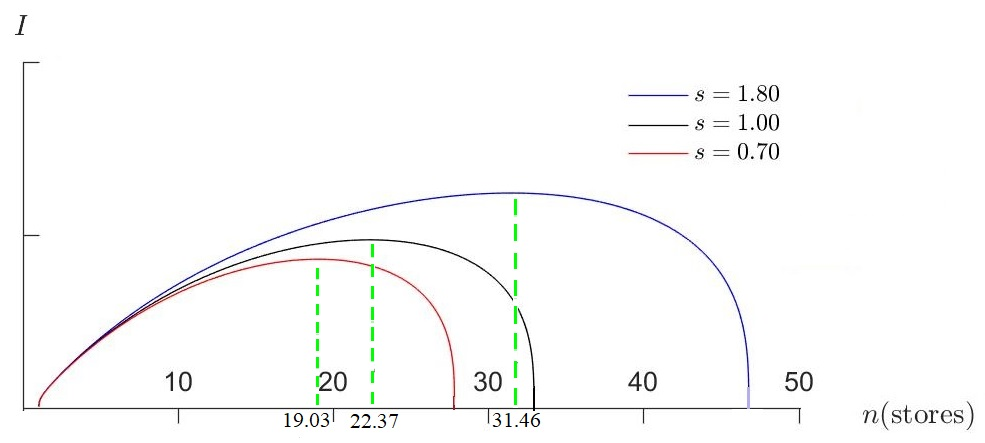
\includegraphics[width=9cm]{sa_mtm_n.jpg}
\caption{the sensitivity of $n$ on $I$}
\label{fig:sa_mtm_n}
\end{figure}

Figure \ref{fig:sa_mtm_n} shows the relationship between $n$ and $I$ under three certain $s$. Obviously $I_{\max}$ is directly related to $n$ under the same $s$, thus proving that our model is effective.

The figure also serves as a virtual show of our model result. The scale will affect $I_{\max}$. It also reveals a truth that the optimal $n$ for each ally varies.

\itembf{the relative scale of the object merchant}

\begin{figure}[H]
\centering
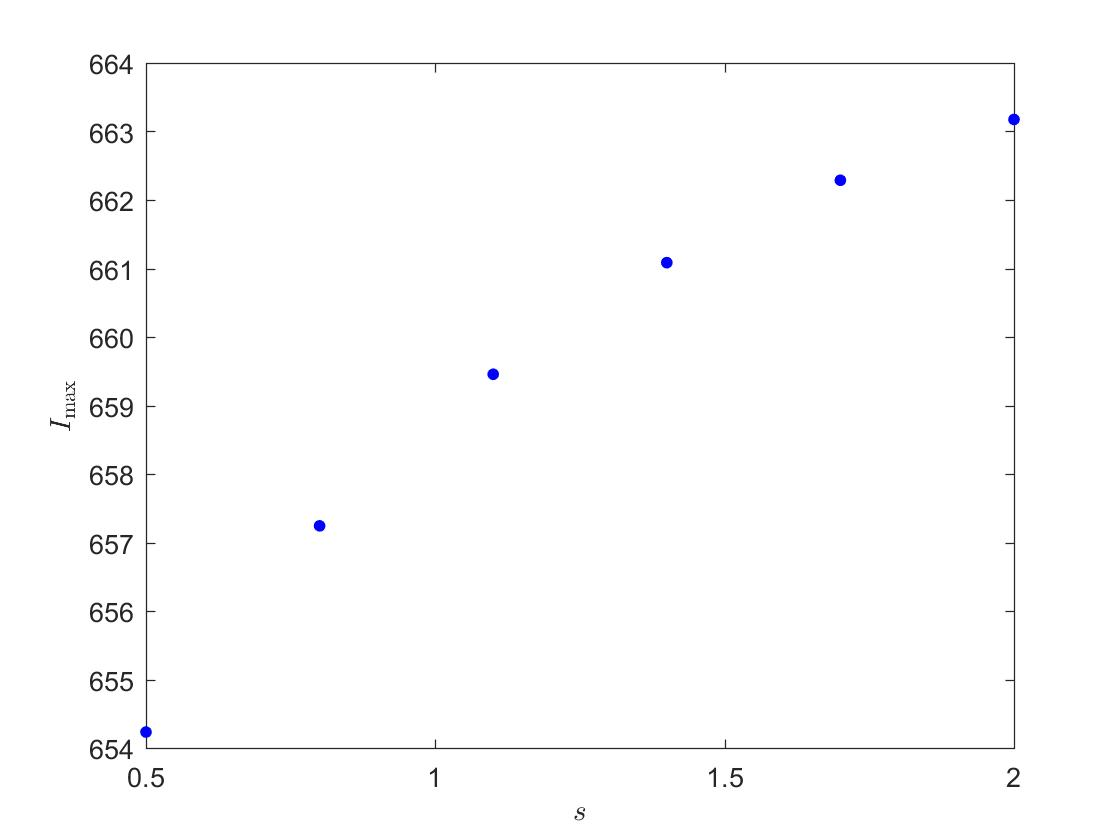
\includegraphics[width=9cm]{sa_mtm_s.jpg}
\caption{the sensitivity of $s$ on $I$}
\label{fig:sa_mtm_s}
\end{figure}

As Figure \ref{fig:sa_mtm_s}\ shows, our model is not sensitive to the relative scale of the object merchant $s$. This indicates that under the same $n$, the business status of the object merchant will not affect its bonus profit, proving that our model is quite robust. And it is worth mentioning that the $n$ in this part of the analysis may not be the optimal $n$ for the object merchant. In fact, it at most time actually isn't.

%\itembf{the overlapping index of all allies to the object merchant}

%\begin{figure}
%\centering
%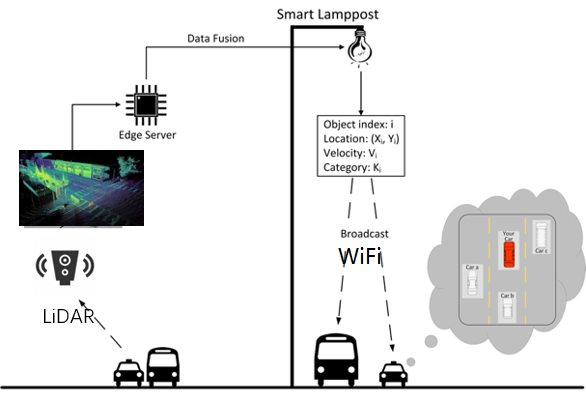
\includegraphics[width=9cm]{mechanism.png}
%\caption{the sensitivity of $\phi$ on $I$}
%\label{fig:sa_mtm_phi}
%\end{figure}

\itembf{the average scale of all allies (\textnormal{the solution to } 2(c))}

\begin{figure}[H]
\centering
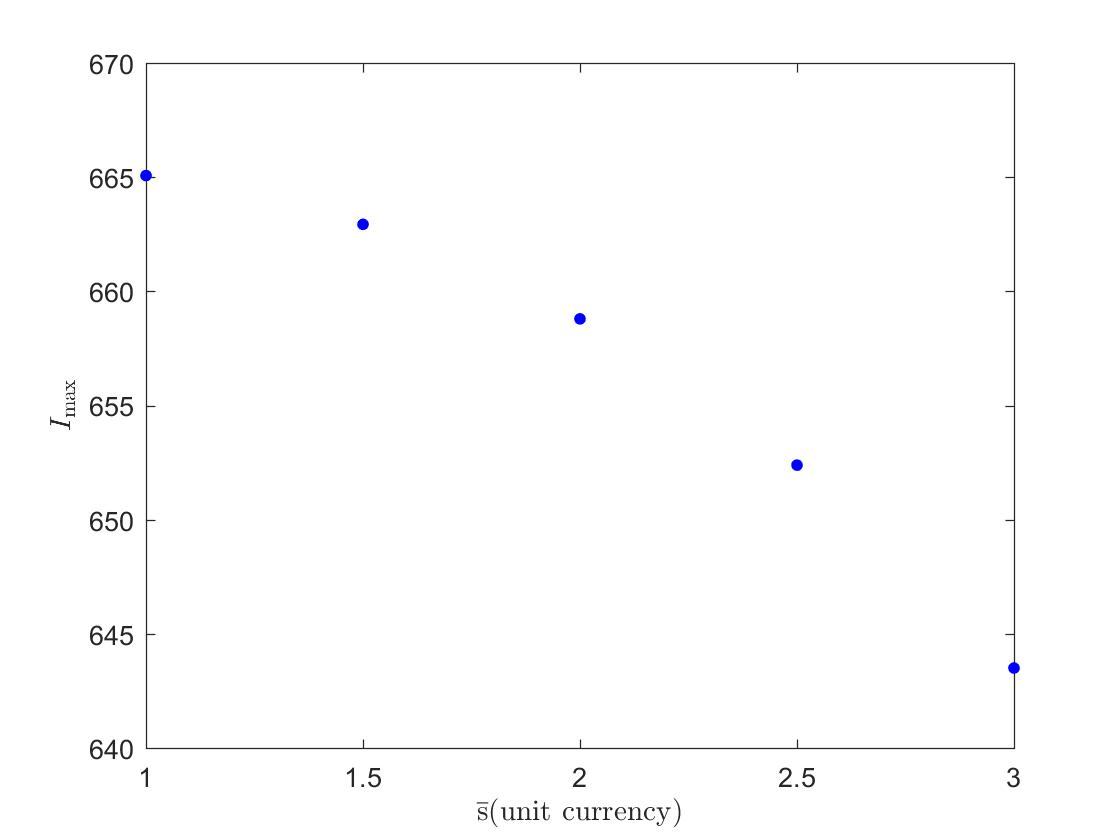
\includegraphics[width=9cm]{sa_mtm_osi.jpg}
\caption{the sensitivity of an $s_i$ on $I$}
\label{fig:sa_mtm_osi}
\end{figure}

In equation \ref{eq:mtm_model}, for the object merchant, $s_1,s_2,\ldots,s_{n-1}$ all serve as constants. So in this part of the sensitivity analysis, we conduct the analysis on one constant $\overline{s_i}$.

The result is that $I$ is not sensitive to $s_i$, meaning that the scale of the allies does not make a difference to the ideal alliance mode. So the change in yearly revenue of allies will not affect our model.

\itembf{the number of Product Type in the universal classification}

\begin{figure}[H]
\centering
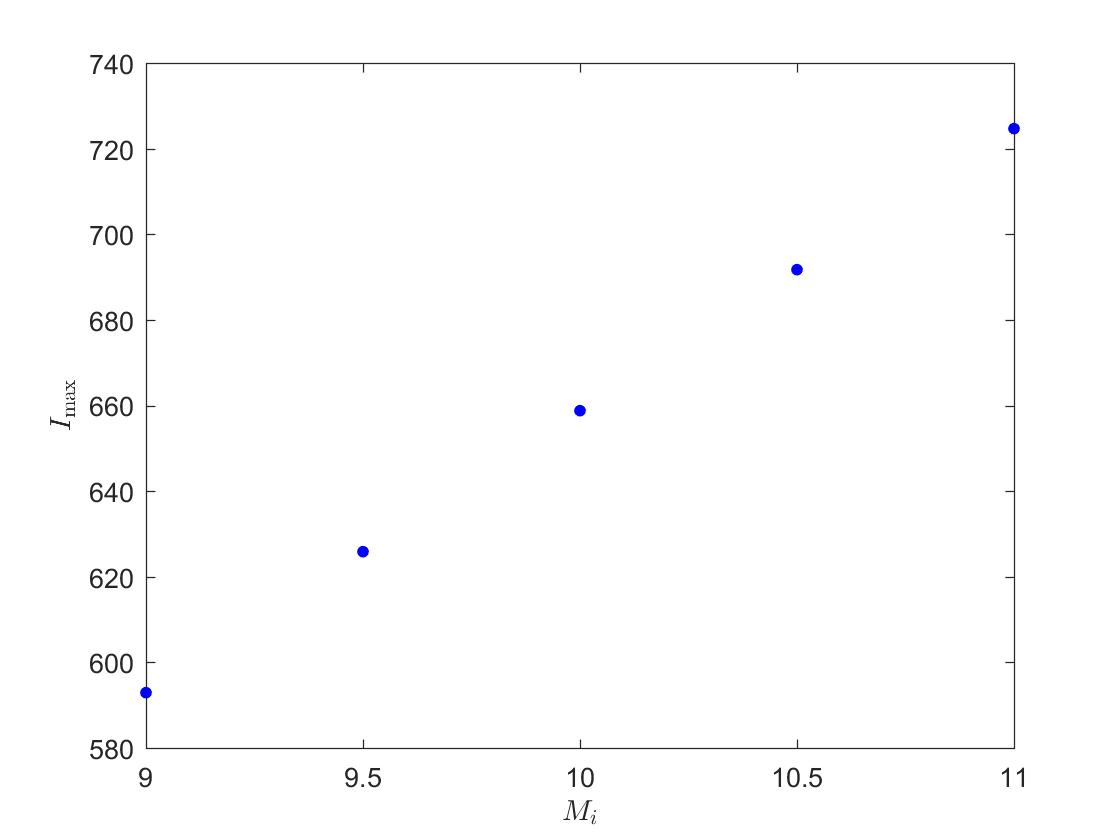
\includegraphics[width=9cm]{sa_mtm_mi.jpg}
\caption{the sensitivity of an $M_i$ on $I$}
\label{fig:sa_mtm_mi}
\end{figure}

Since $M_i$ indicated the resolution of the product type classification, its size should only affect the accuracy of the $I_{\max}$. However, our model is relatively quite sensitive to $M_i$, making it fragile.
\end{enumerate}